\section{Durchführung}
\label{sec:Durchführung}
Der Aufbau des Versuches ist in folgender Abbildung schematisch dargestellt.
  \begin{figure}[H]
    \centering
      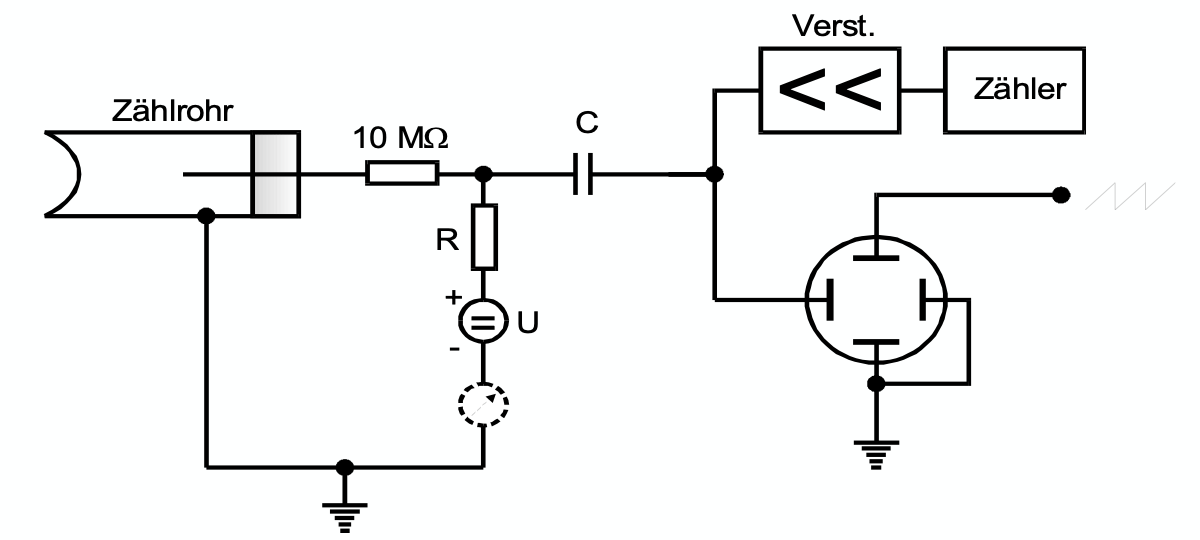
\includegraphics[scale=0.6]{content/AufbauV703.png}
      \caption{Der Versuchsaufbau. Quelle:\cite{AP01}}
      \label{fig:aufbau3}
  \end{figure}
\label{sec:Durchführung}
\noindent
Die Ladung $Q$, die auf dem Zähldraht innerhalb des Zählrohres aufgenommen wird, fließt über den
Widerstand $R$. Dabei entsteht eine Spannung, die mit dem Kondensator ausgekoppelt und dann mithilfe
des Verstärkers vergößert wird. Die vergößerte Spannung wird dann mit dem Oszillographen sichtbar
gemacht. In Schritten von $\increment U = 10 \si{\volt}$ wurde die Anzahl Zerfälle innerhalb eines
Zeitintervalls aufgenommen. Um sicherzustellen, dass die Totzeit die Messung nicht beeinflusst,
wurde mit einer Integrationszeit von $t = 60 \si{\second}$ gearbeitet. Der Zählrohrstrom wird alle
$\SI{50}{\volt}$ am Amperemeter abgelesen. 
